\newpage
\subsection{The microcontroller}

\begin{figure}[!h]
    \centering
    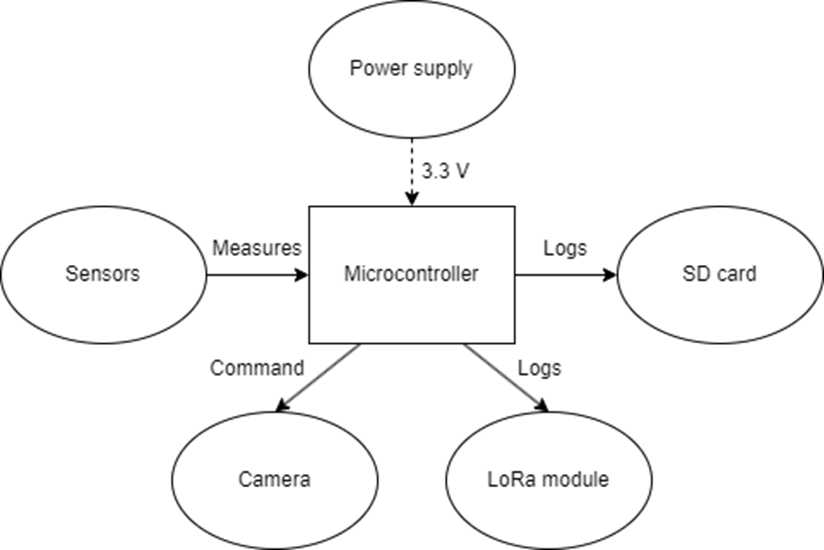
\includegraphics[width=0.8\textwidth]{\currfiledir/figures/micro.png}
    \caption{Schematic of the microcontroller and its relationships with other elements}
\end{figure}

The microcontroller is the core of the device. It is responsible to command the whole system. The STM32 Nucleo F303K8 microcontroller was chosen for this project due to several key features that make it suitable for our application. Firstly, it has very low power consumption, with only 3mA in sleep mode and 13mA during operation. Secondly, it includes a built-in Real-Time Clock (RTC), eliminating the need for an external RTC module, thereby saving cost and board space. Furthermore, one was readily available, which saved time and reduced the overall project cost.\\
The microcontroller operates on a 3.3V power supply, a common voltage level for many electronic devices, simplifying integration into our project without the need for additional voltage regulation or level shifting circuits. This compatibility allows for seamless connections with the various sensors in our system, such as the ICM-20602 motion sensor, the AM2320 humidity and temperature sensor, the LM35DZ internal case temperature sensors, and the TSL2561 light sensor. The microcontroller receives data from these sensors and processes it to make decisions and execute predefined actions, ensuring the proper functioning of the system.\\
Lastly, the STM32 Nucleo F303K8 microcontroller offers multiple communication interfaces, such as I2C, SPI, and UART, providing flexibility in connecting and communicating with the sensors and other peripherals, like the LoRa module, in our project. These interfaces facilitate the efficient transmission of sensor data to the microcontroller for real-time monitoring, analysis, and response.\\
The microcontroller is being programmed in order to use the temperature and humidity sensor, and the SD card in order to create logs.
